\chapter{Resultados y discusión}

\section{Caracterización de la RI sin neoprene} 

\subsection{Comparación entre las mediciones y el modelo COMSOL}

Los modelos realizados en COMSOL muestran la respuesta en frecuencias del acuario en toda su extensión. Para condiciones de borde suaves los primeros modos normales son los debidos al bloque de agua y concuerdan con las primeras frecuencias aproximadas por la ecuación \ref{eq:resonancias}, de $\approx 6200\pm10$Hz con las medidas del acuario. En las figuras \ref{subfig:comsolsuave} y \ref{subfig:comsolmedio} se pueden observar gráficos de la respuesta en frecuencia calculada por COMSOL para un punto de la pecera utilizando las dos condiciones de borde explicadas en la introducción: todos bordes suaves, y condición de impedancia. Para el primer tipo de condiciones de borde sólo se observan modos de frecuencias superiores a 6kHz, mientras que en el segundo se observan algunos de baja intensidad en casi todo el rango estudiado. En todas las simulaciones la presión total de la onda emitida por el parlante es de 1Pa.

\begin{figure}[H]
	\begin{subfigure}[b]{.49\textwidth}
		\centering
			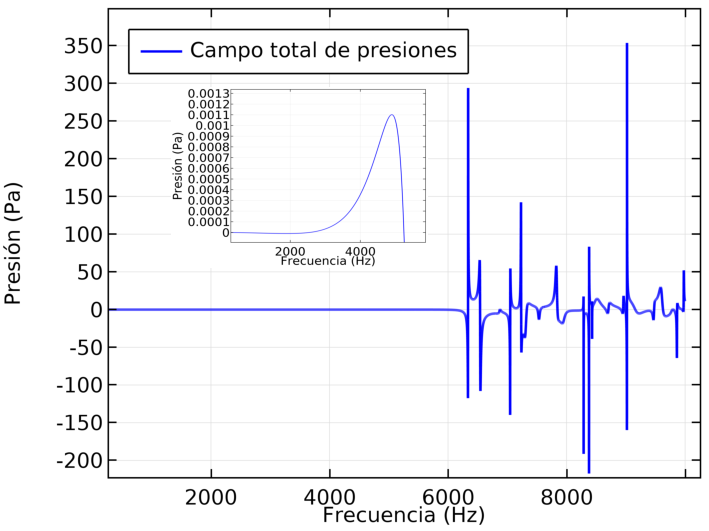
\includegraphics[width=\textwidth, height=4cm]{presiones1.pdf}
			\caption{Bordes suaves.}
			\label{subfig:comsolsuave}
	\end{subfigure}
	\hfill
	\begin{subfigure}[b]{.49\textwidth}
		\centering
			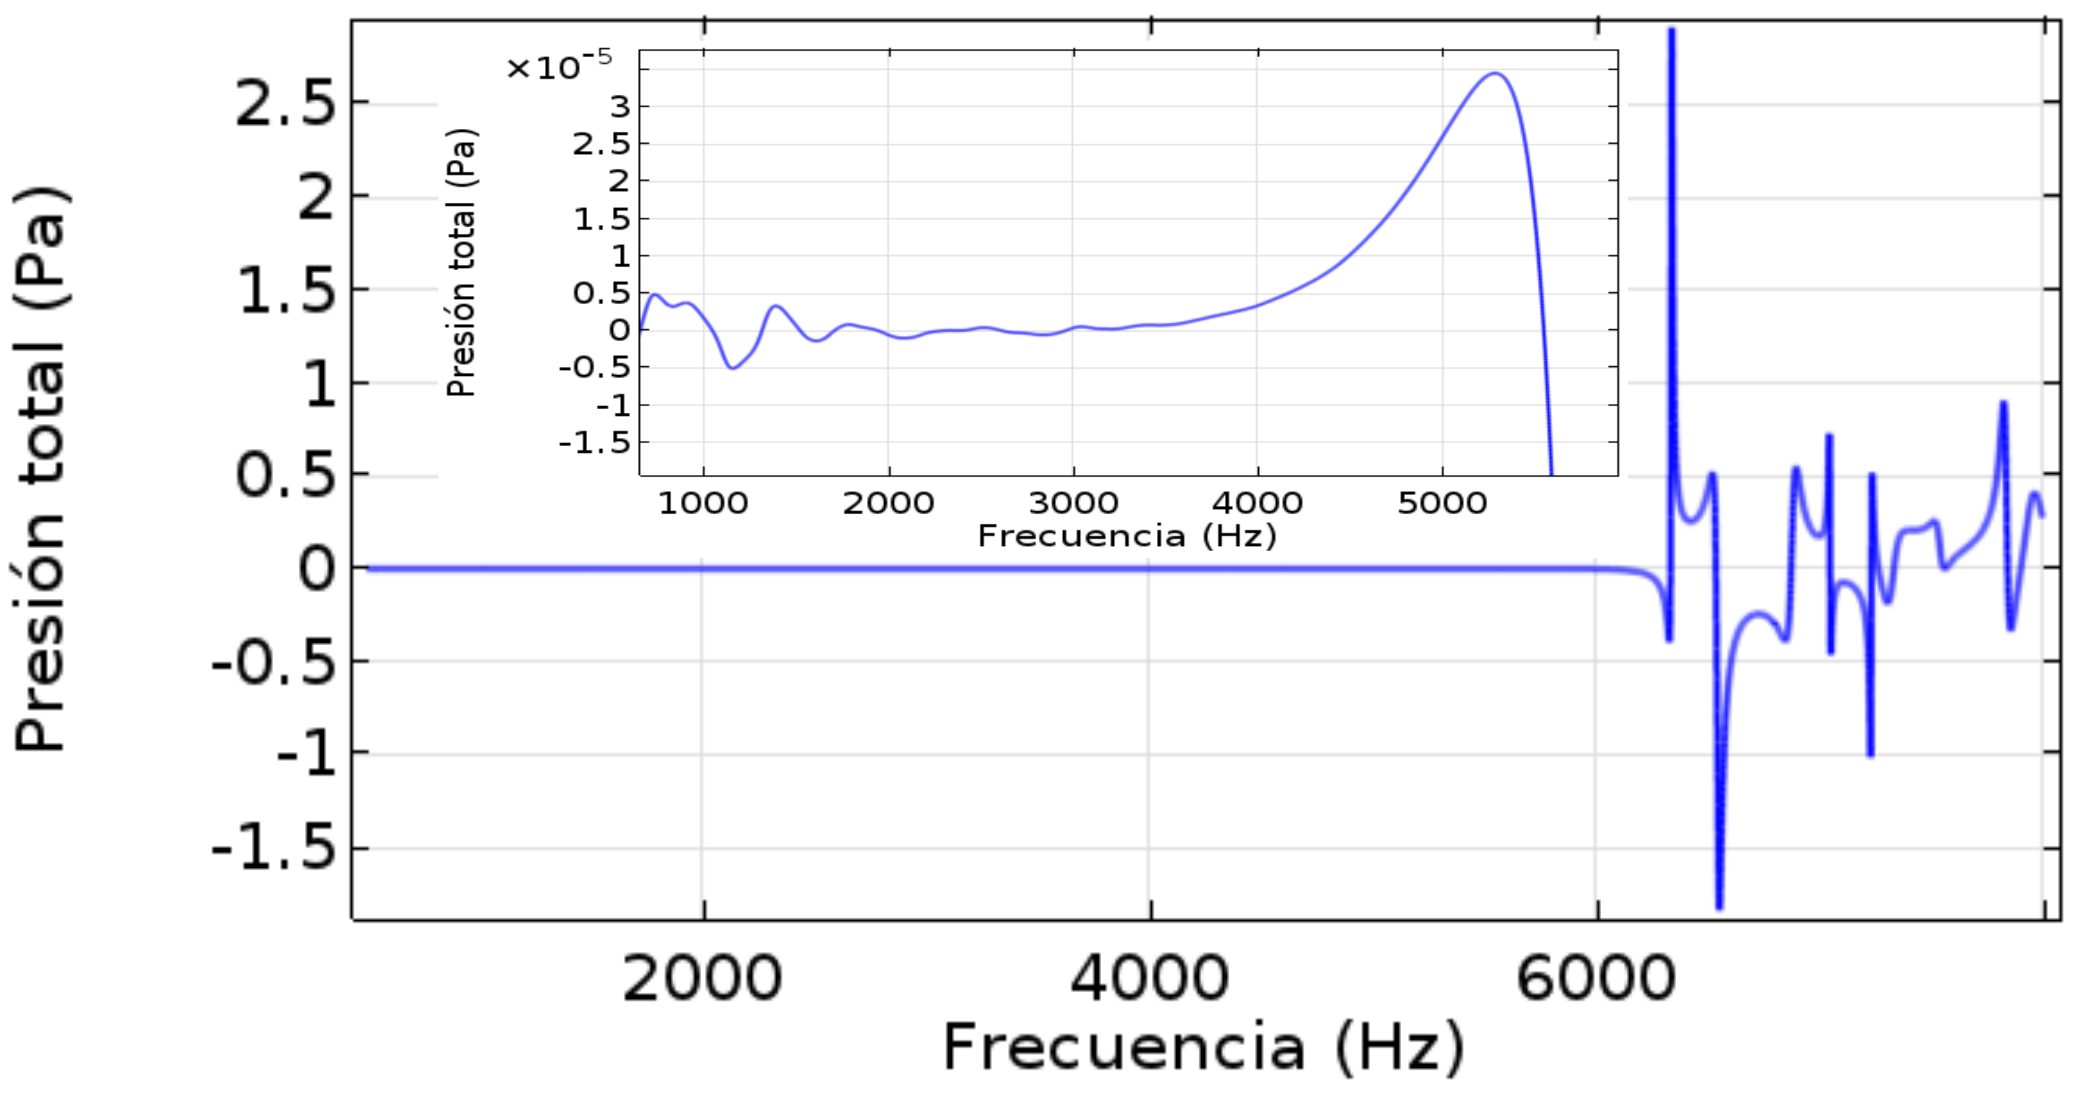
\includegraphics[width=\textwidth, height=4cm]{frcomsol.png}
			\caption{Condición de impedancia.}
			\label{subfig:comsolmedio}
	\end{subfigure}
	\caption{Respuesta en frecuencias del acuario calculada por COMSOL.}
	\label{fig:frcomsol}
\end{figure}

En las RI medidas los modos de alta frecuencia sólo aparecen en la mitad de la pecera más alejada del parlante (el parlante sólo excita esos modos en esa mitad del acuario). En todo el acuario, sin embargo, se observan los modos de bajas frecuencias. En las figuras \ref{subfig:x1y34}, \ref{subfig:x1y34zoom}, \ref{subfig:x7y34} y \ref{subfig:x7y34zoom} se muestran las RIs medidas en distintos puntos de las dos mitades de la pecera. Allí, todos los modos normales se ven como barras horizontales de gran intensidad.

\begin{figure}[H]
		\begin{subfigure}[b]{\textwidth}
			\centering
			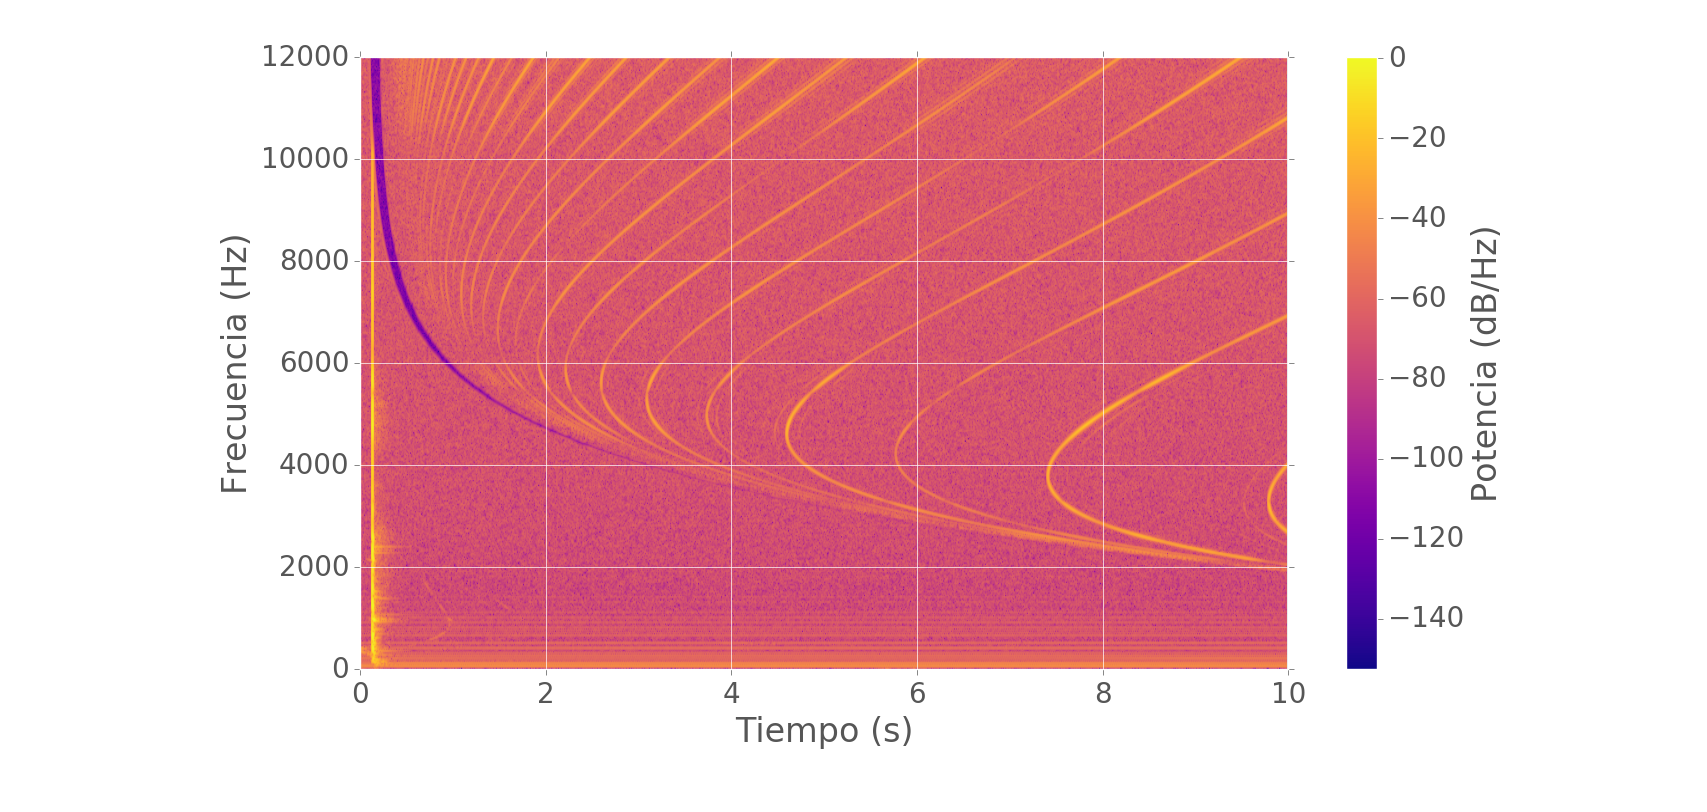
\includegraphics[width=\textwidth]{x1y34.png}
			\caption{RI completa.}
			\label{subfig:x1y34}
		\end{subfigure}

		\begin{subfigure}[b]{\textwidth}
			\centering
			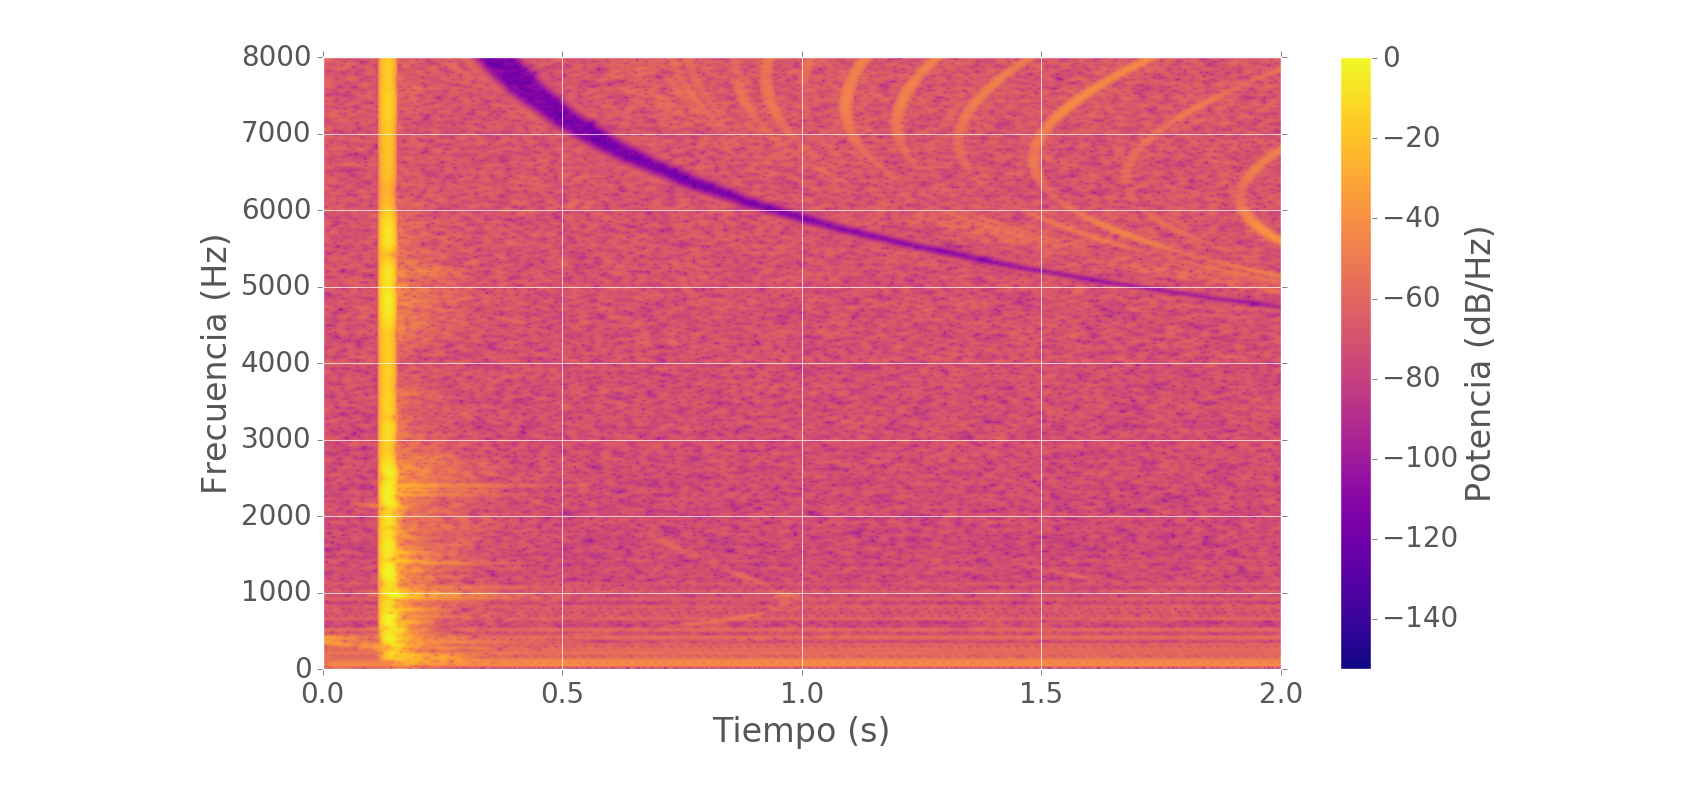
\includegraphics[width=\textwidth]{x1y34zoom.png}
			\caption{Detalle de \ref{subfig:x1y34}.}
			\label{subfig:x1y34zoom}
		\end{subfigure}
		\caption{RI en la primer mitad de la pecera donde se observan los modos de baja frecuencia. Las franjas violetas son artefactos causadas por el método de deconvolución-}
		\label{fig:modosbajos1}
\end{figure}

\begin{figure}[H]
		\begin{subfigure}[b]{\textwidth}
			\centering
			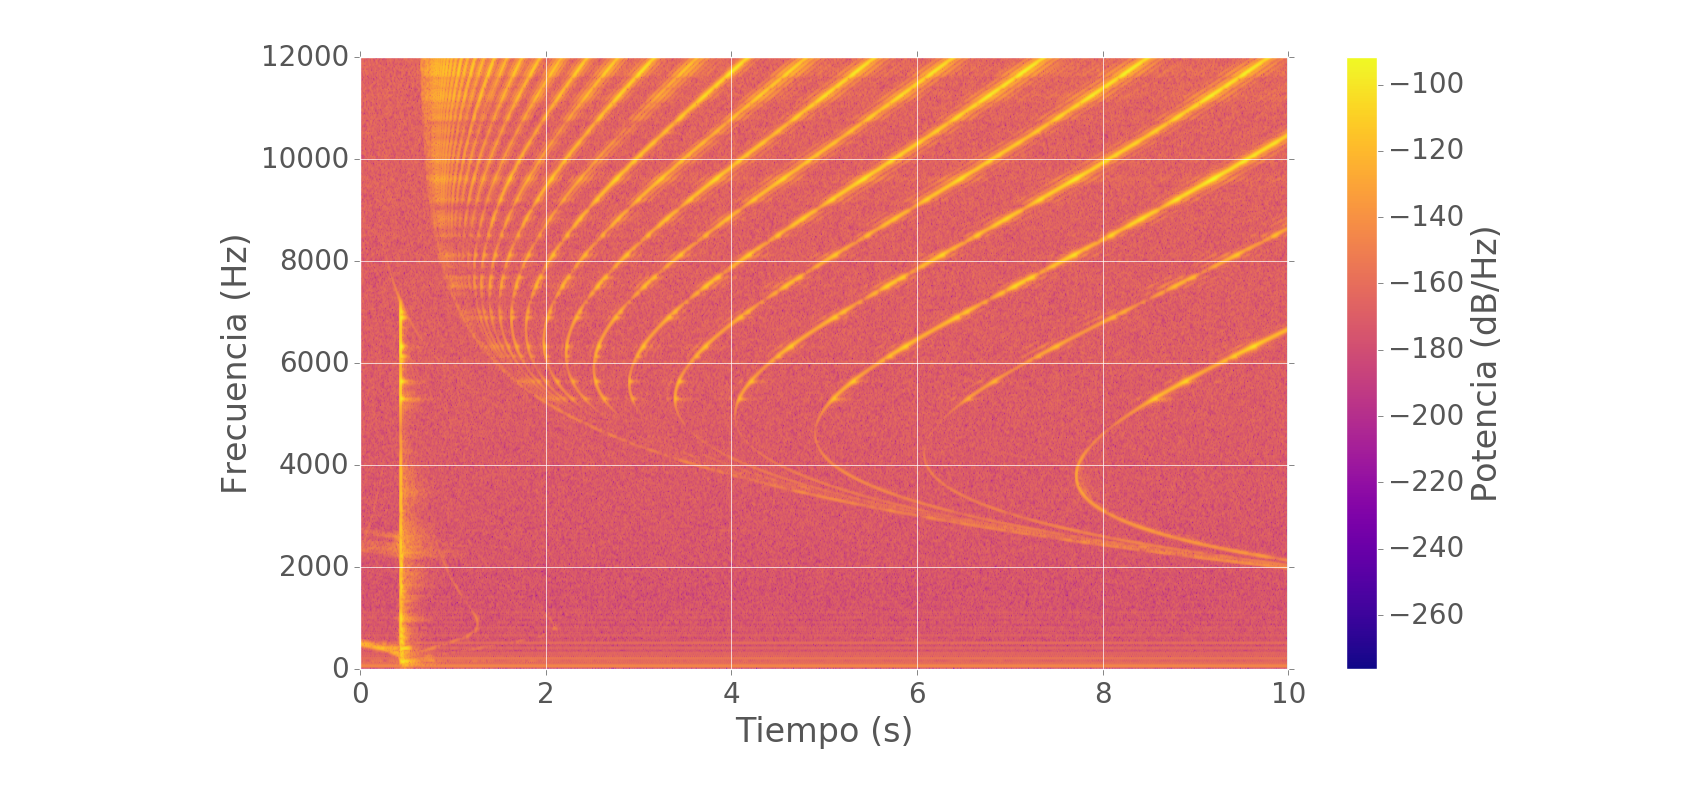
\includegraphics[width=\textwidth]{x7y34.png}
			\caption{RI completa.}
			\label{subfig:x7y34}
		\end{subfigure}

		\begin{subfigure}[b]{\textwidth}
			\centering
			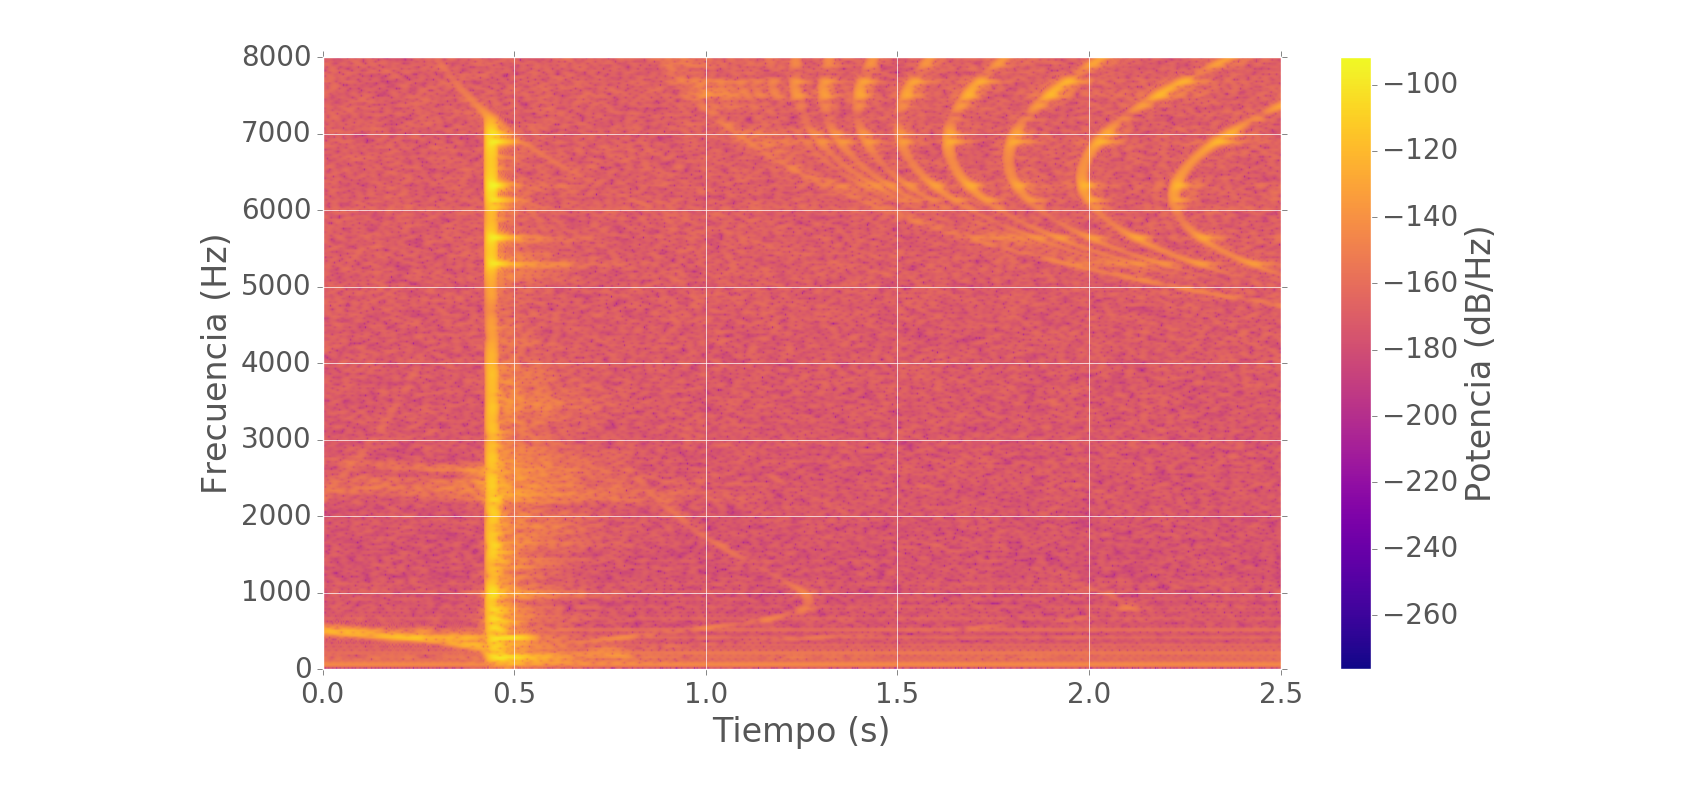
\includegraphics[width=\textwidth]{x7y34zoom.png}
			\caption{Detalle de \ref{subfig:x7y34}.}
			\label{subfig:x7y34zoom}
		\end{subfigure}
		\caption{RI en la segunda mitad de la pecera donde se observan los modos de baja y alta frecuencia.}
		\label{fig:modosaltos1}
\end{figure}

Los resultados obtenidos indican que las condiciones de borde más acordes a la realidad son aquellas en que la superficie libre se modela a partir del cambio de impedancias. En principio, para obtener una predicción completa de todos los campos involucrados es necesario incluir en COMSOL un modelo de emisión del parlante (si bien los modos son propios de la pecera, el parlante puede excitar distintos modos en distintos puntos).

\subsection{Patrones y direccionalidad del campo de presiones}
\label{sec:rescompo}

\begin{figure}[H]
	\begin{subfigure}[b]{.48\textwidth}
		\centering
		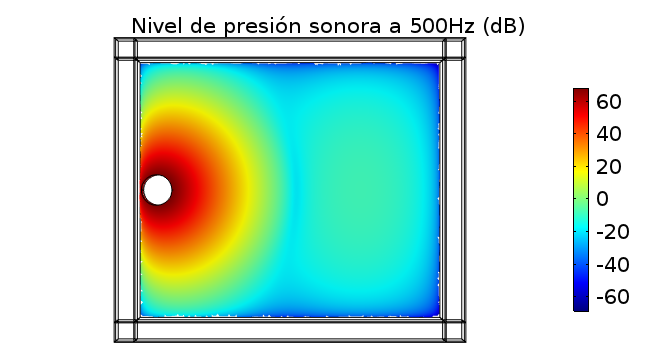
\includegraphics[width=\textwidth , height=4cm]{comsolcampo1.png}
	\end{subfigure}
	\begin{subfigure}[b]{.48\textwidth}
		\centering
		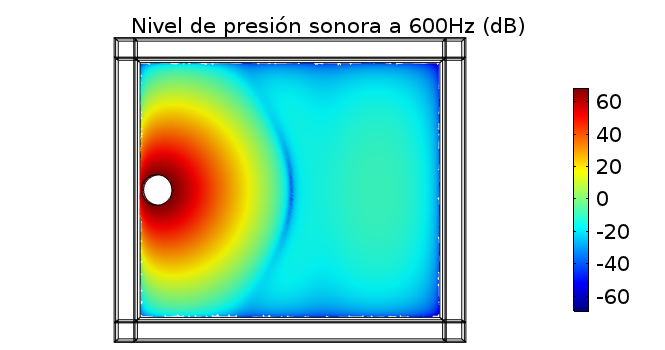
\includegraphics[width=\textwidth , height=4cm]{comsolcampo2.png}
	\end{subfigure}
	
	\begin{subfigure}[b]{.48\textwidth}
		\centering
		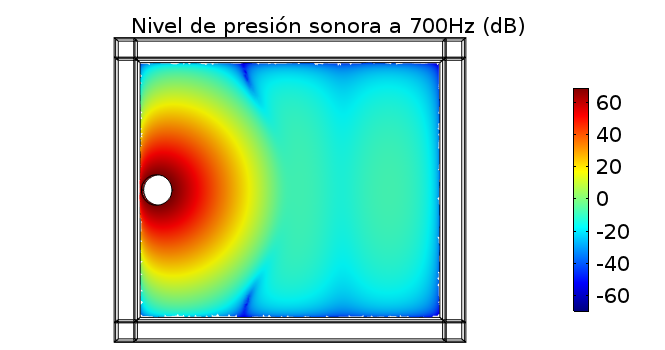
\includegraphics[width=\textwidth , height=4cm]{comsolcampo3.png}
	\end{subfigure}
	\begin{subfigure}[b]{.48\textwidth}
		\centering
		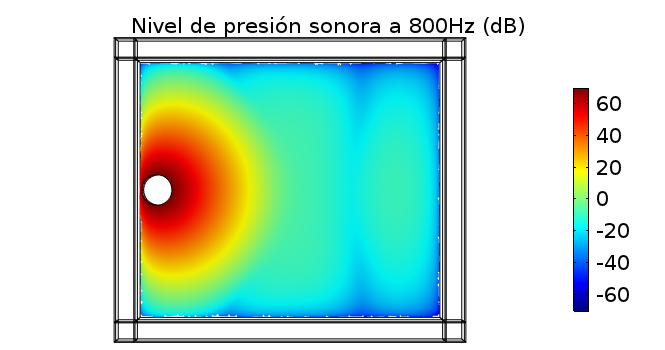
\includegraphics[width=\textwidth , height=4cm]{comsolcampo4.png}
	\end{subfigure}
	
	\begin{subfigure}[b]{.48\textwidth}
		\centering
		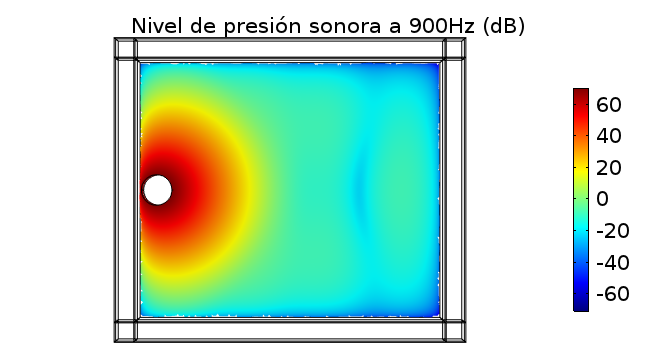
\includegraphics[width=\textwidth , height=4cm]{comsolcampo5.png}
	\end{subfigure}
	\begin{subfigure}[b]{.48\textwidth}
		\centering
		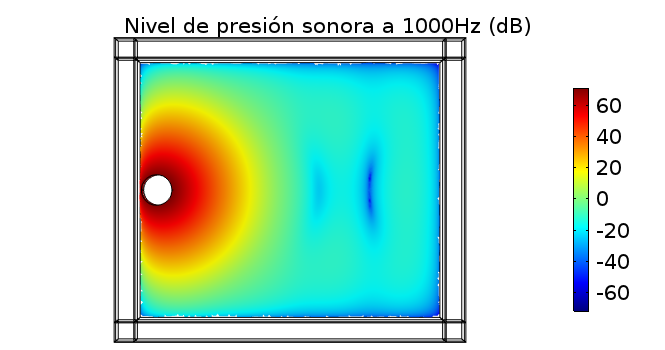
\includegraphics[width=\textwidth , height=4cm]{comsolcampo6.png}
	\end{subfigure}
	
	\begin{subfigure}[b]{.48\textwidth}
		\centering
		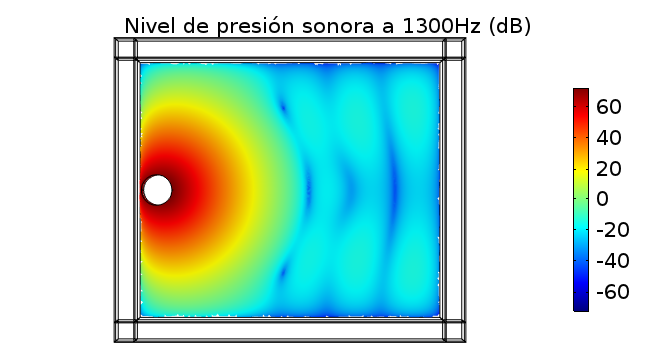
\includegraphics[width=\textwidth , height=4cm]{comsolcampo7.png}
	\end{subfigure}
	\begin{subfigure}[b]{.48\textwidth}
		\centering
		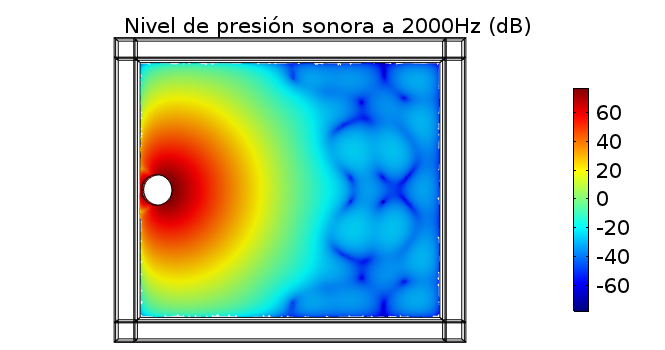
\includegraphics[width=\textwidth , height=4cm]{comsolcampo8.png}
	\end{subfigure}
	\caption{Campos de presiones calculados por COMSOL en toda la pecera.}
	\label{fig:campos}
\end{figure}

Para decidir en qué zonas de la pecera se realizarán los experimentos, es necesario observar en el modelo COMSOL cómo son los patrones del campo de presiones para distintas frecuencias. Los resultados del modelo muestran que en la primer mitad del acuario la direccionalidad del campo de presiones está bien definida para todos los modos y es hemiesférica hacia adelante. En la segunda mitad, los modos de bajas frecuencias forman patrones irregulares donde la direccionalidad no es clara: en esa zona no deberían realizarse experimentos comportamentales, ya que no se puede inferir la direccionalidad del estímulo. La figura \ref{fig:campos} muestra los patrones del campo de presiones a distintas frecuencias.

\section{Caracterización de la RI con neoprene}

A raíz de su uso como aislante en aire y su resistencia al agua, se decidió utilizar neoprene como aislante y delimitador de la zona en la que se realicen los experimentos con animales. Sin embargo la velocidad de propagación del sonido en neoprene es muy cercana a la del agua, y el material es casi invisible en lo que respecta a la acústica a bajas frecuencias. A altas frecuencias, el material podría, a lo sumo, interactuar en forma poroacústica. En las figuras \ref{subfig:neoprene1} y \ref{subfig:neoprene2} se pueden observar dos espectrogramas de la RI medida con neoprene en los mismo puntos de las figuras \ref{fig:modosbajos1} y \ref{fig:modosaltos1}.

\begin{figure}[H]
	\begin{subfigure}[b]{\textwidth}
		\centering
		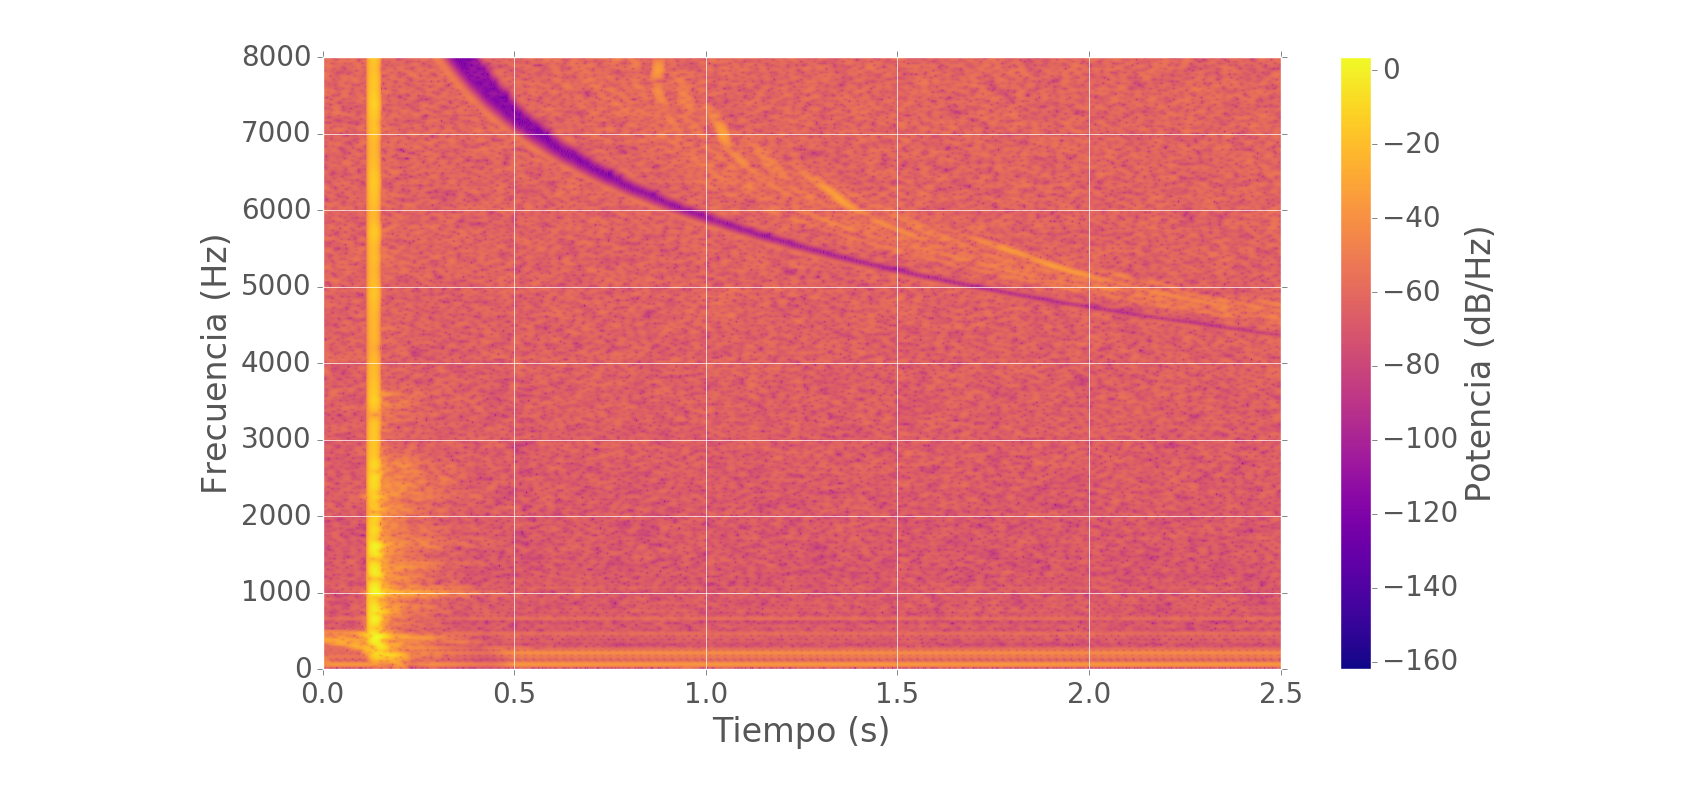
\includegraphics[width=\textwidth , height=6cm]{x1y34neo.png}
		\caption{Primera mitad de la pecera.}
		\label{subfig:neoprene1}
	\end{subfigure}

	\begin{subfigure}[b]{\textwidth}
		\centering
		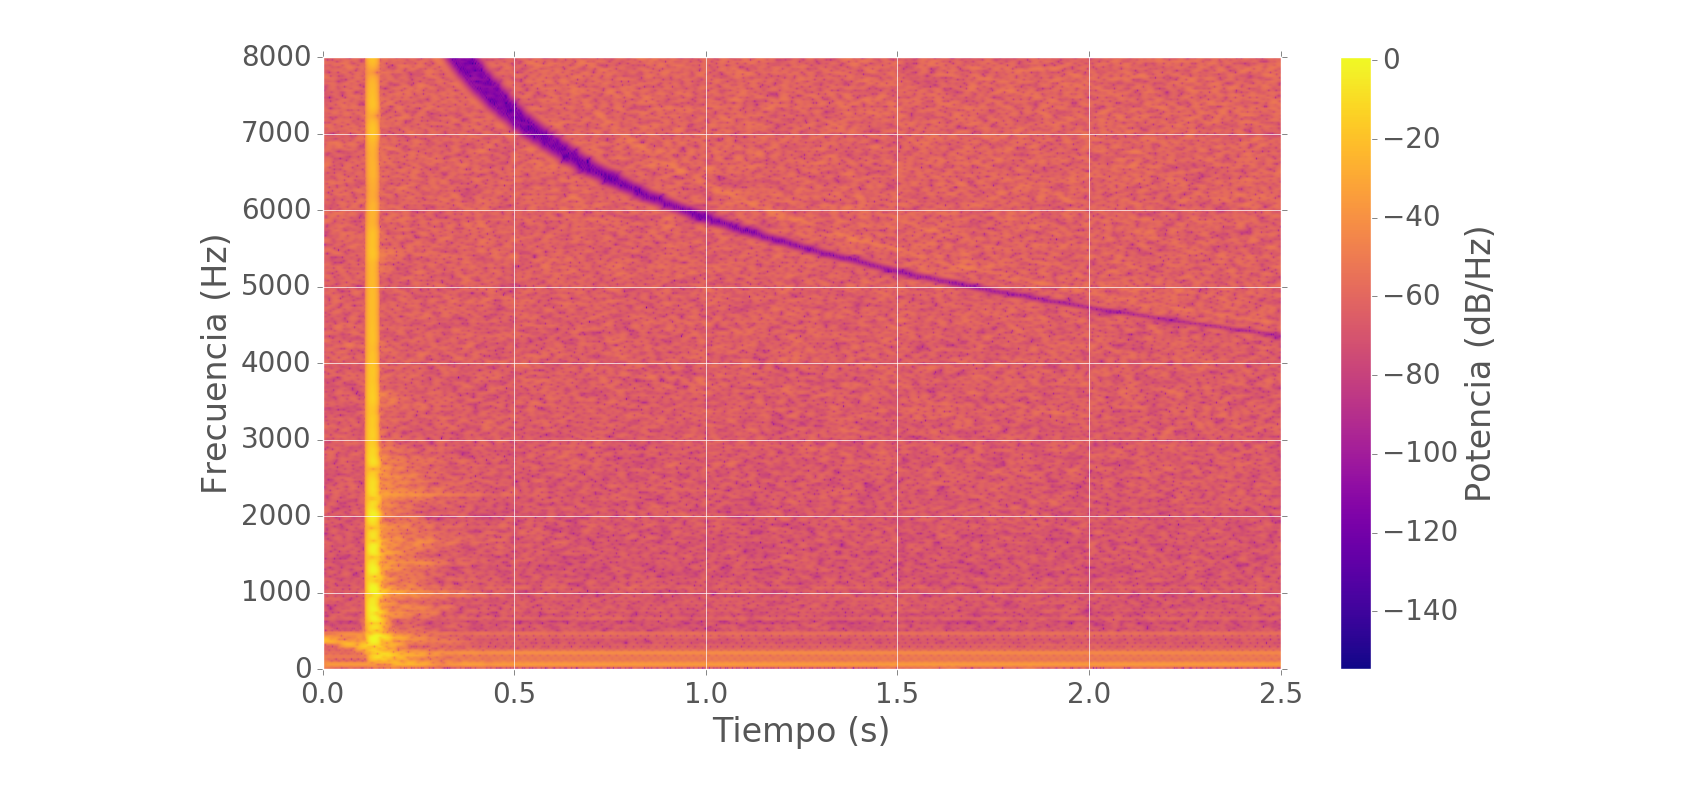
\includegraphics[width=\textwidth , height=6cm]{x7y34neo.png}
		\caption{Segunda mitad de la pecera.}
		\label{subfig:neoprene2}
	\end{subfigure}
	\caption{RI medida con neoprene. Las franjas violetas son artefactos causados por el método de deconvolución.}
\end{figure}

Se realizaron mediciones adicionales utilizando en la configuración de la figura \ref{fig:conneobis}. Esta última configuración fué utilizada para delimitar como zona experimental a la primer mitad del acuario, en la cual se realizaron lo estudios comportamentales. Al no observar cambios cualitativos apreciables en la RI salvo una baja en la intensidad de los modos excitados, se decidió no modelar sus propiedades en COMSOL. Esto puede hacerse si se miden propiedades del material (coeficientes de absorción, módulo de Young, etc.) y se programa al material en COMSOL, ya que el mismo no tiene goma de neoprene en ninguna de sus librerías. 

\section{Experimentos comportamentales}

Con la zona experimental delimitada por el neoprene, se realizaron experimentos comportamentales utilizando los estímulos de la tabla \ref{tab:estimulos}. Tanto para barridos como tonos puros, se observa siempre un aumento en la frecuencia de descarga de la DOE (i. e. disminuye el tiempo entre descargas). La figura \ref{fig:doemiedo} muestra gráficos del tiempo entre descargas y de la DOE misma en función del tiempo de medición.

\begin{figure}[H]
	\centering
		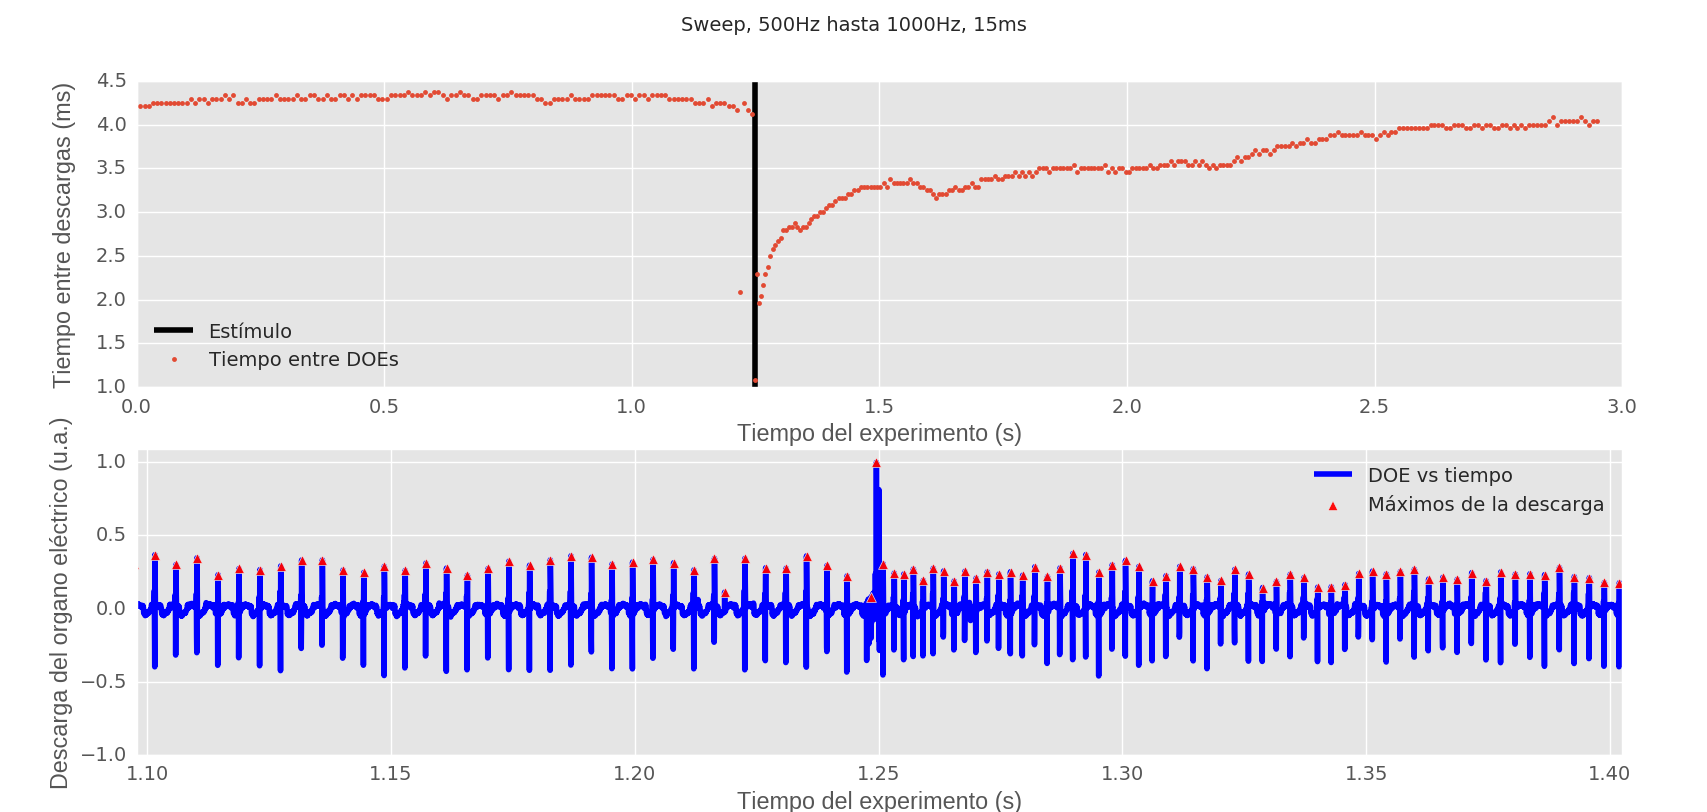
\includegraphics[width=\textwidth]{sw6.png}
	\caption{DOE y tiempo entre descargas. Cada pico marcado con un triángulo rojo es una descarga. Los errores de medición se han tomado como el promedio del ancho mitad de la DOE y son del orden de 0,2ms. El tiempo entre descargas se calcula restando los tiempos entre picos adyacentes.}
	\label{fig:doemiedo}
\end{figure}

En las tablas \ref{tab:rescompo} se muestran los resultados obtenidos con cada estímulo. Se han tenido en cuenta el cambio de tiempo entre descargas al momento del estímulo, $\Delta DOE$, y el tiempo que tarda el animal en volver a su frecuencia basal (tiempo entre descargas antes del estímulo), $\Delta_b$. Si bien el número de mediciones realizadas no permite realizar estadística en cuanto a qué tipo de estímulo es mejor, si se pueden obtener algunos datos útiles:
\begin{itemize}
	\item En todos los casos, el tiempo que tarda el animal en volver a la frecuencia basal es por lo menos dos ordenes de magnitud mayor que la duración del estímulo (y el tiempo entre descargas).
	\item A priori la única diferencia observable a simple vista es que los barridos producen cambios más grandes en la frecuencia de la DOE y tiempos más largos en volver a la frecuencia basal.
\end{itemize}
\newpage
\begin{table}[H]
\centering
%\resizebox{\textwidth}{!}{%
\begin{tabular}{c|c|c}
\doublerule
Estímulo & $\Delta DOE$ (ms) & $\Delta_b$ (s) \\	\midrule
Sweep 1  & 2.2               & 1.1            \\
Sweep 2  & 0.8               & 1.5            \\
Sweep 3  & 1.5               & 1.7            \\
Sweep 4  & 0.4               & 1.4            \\
Sweep 5  & 0.8               & 1.1            \\
Sweep 6  & 2.4               & 2.7            \\
Sweep 7  & 0.6               & 2.3            \\
Sweep 8  & 1.7               & 0.4            \\
Sweep 9  & 0.9               & 2.0            \\
Sweep 10 & 0.4               & 1.0            \\	\midrule
Tono 1   & 0.9              & 1.8            \\
Tono 2   & 0.9               & 1.5            \\
Tono 3   & 0.3               & 0.1            \\
Tono 4   & 0.8               & 0.7            \\
Tono 5   & 1.6               & 0.9            \\
Tono 6   & 0.8               & 0.6            \\
Tono 7   & 1.4               & 1.0            \\
Tono 8   & 1.7               & 1.0            \\
Tono 9   & 0.9               & 0.9            \\
Tono 10  & 0.5               & 0.8            \\	\bottomrule 
\end{tabular}%
%}
\caption{Resultado obtenidos para cada estímulo. Se muestran las disminuciones en los tiempos entre descargas y el tiempo que tarda el animal en volver a la frecuencia basal.}
\label{tab:rescompo}
\end{table}
